\section{How Concentrated Liquidity Works}
\label{sec:background}

\subsection{A position as a bet on a range}

Uniswap~v3 indexes price by integer ticks. An LP picks a lower and an upper
tick, and the deposit backs trades only while the pool price stays between
them\cite{adams2021uniswap}. In protocol units the price is a raw square root,
$s=\sqrt{1.0001^{\text{tick}}}$, which increases with the tick; the human price
is $q(s)=10^{d_1-d_0}/s^2$ USDC per WETH, so a lower tick means a higher ETH
price. Inside a band $[s_a,s_b]$ the position holds the token amounts
\begin{align}
x(s) &= \frac{L}{10^{d_0}}\left(\frac{1}{s}-\frac{1}{s_b}\right),
\label{eq:x}\\
y(s) &= \frac{L}{10^{d_1}}\left(s-s_a\right),
\label{eq:y}
\end{align}
and its USDC value is therefore
\begin{equation}
V(s) = x(s) + y(s)\,q(s)
     = \frac{L}{10^{d_0}}\left(\frac{2}{s}-\frac{1}{s_b}-\frac{s_a}{s^2}\right).
\label{eq:value}
\end{equation}
As the ETH price falls, the position sells USDC and accumulates WETH; as the
price rises it does the opposite. At an edge of the band the position holds a
single asset, and once the price leaves the band it stops trading altogether,
so a passive position cannot escape the wrong side of a move.

Fees accrue in proportion to the position's share of active liquidity.
Narrowing the band raises that share for a given deposit, which is why
concentration is attractive, but it also shortens the expected time until the
price reaches an edge. That tension between fee density and band lifetime sits
underneath every decision in the report, and Fig.~\ref{fig:payoff} shows the
two effects together.

\begin{figure}[tbp]
\centering
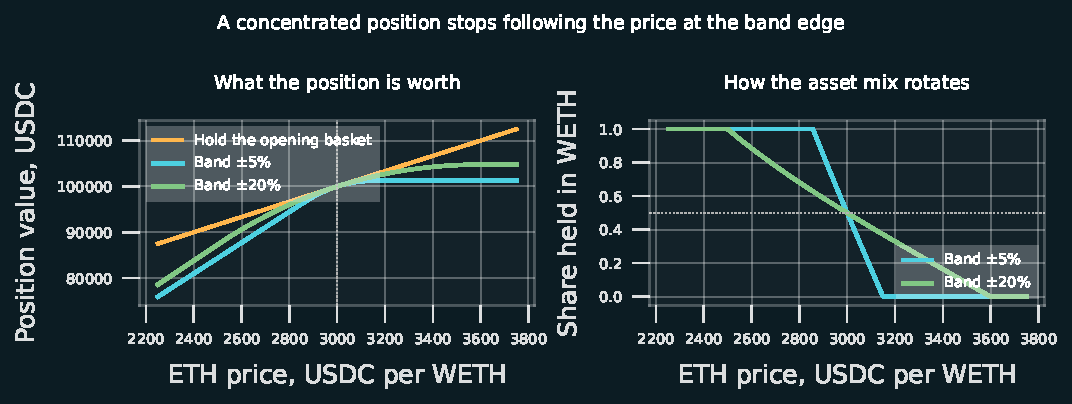
\includegraphics[width=0.92\linewidth]{figures/position_payoff.pdf}
\caption{A concentrated position versus a passive holding of the same opening
basket. Left: the position tracks the basket while the price sits inside the
band and stops following it at the edges, so it gives up the upside of a rally
while keeping the downside of a fall. Right: the asset mix rotates from WETH
to USDC as the price rises and freezes at the edge. Illustrative parameters:
\usdc{100000} entered at \SI{3000}{USDC} per WETH.}
\label{fig:payoff}
\end{figure}

\subsection{Two losses, one larger}

Impermanent loss (IL) is the shortfall of the position against holding the
initial deposit. For a full-range position with equally valued legs and price
ratio $r=q_t/q_0$,
\begin{equation}
\mathrm{IL}(r) = \frac{2\sqrt{r}}{1+r} - 1,
\label{eq:il}
\end{equation}
which is second order in the price move; at $r=1.2$ it is $-0.41\,\%$. On v3
the same expression applies only inside the band, and outside it the position
is a one-sided holding, so IL depends on where the band was
placed\cite{loesch2021impermanent}.

LVR is sharper. Compare the position with a portfolio that continuously
rebalances to hold the same instantaneous exposure. A second-order expansion of
the full-range value shows that the LP falls behind that portfolio at the rate
\begin{equation}
\mathrm{dLVR}_t = \frac{1}{8}\,\sigma^2\,V_t\,\mathrm{d}t,
\label{eq:lvr}
\end{equation}
the loss-versus-rebalancing of Milionis et al.\cite{milionis2022lvr}. Adverse
selection therefore grows with the square of volatility and with position size,
and fee income must exceed it for passive provision to be viable. Concentration
raises fee density but not the fee rate, so it helps only when the extra fee
share outweighs the extra exposure to arbitrage; Section~\ref{sec:related}
finds that on many large pools it does not. Figure~\ref{fig:losses} shows the
shape of both losses.

\begin{figure}[tbp]
\centering
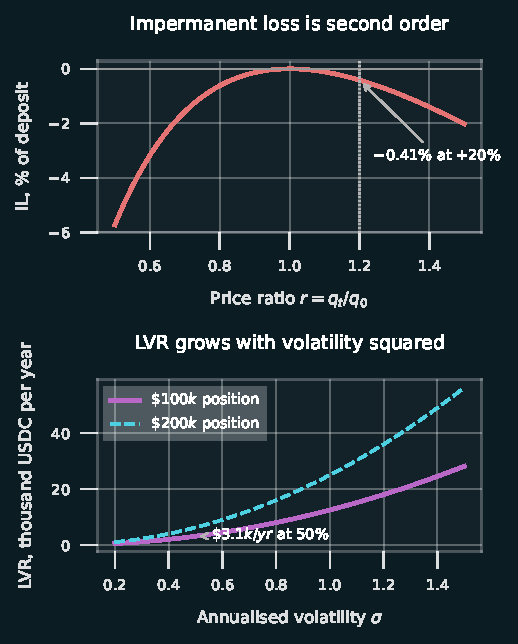
\includegraphics[width=0.55\linewidth]{figures/il_lvr.pdf}
\caption{The two losses. Top: impermanent loss against the price move, second
order and small for a full-range position. Bottom: the LVR rate against
volatility for a \usdc{100000} and a \usdc{200000} position, showing both the
quadratic dependence on volatility and the linear dependence on size.}
\label{fig:losses}
\end{figure}

\subsection{The decisions and the risk}

An LP that wants to improve on the passive outcome must decide when to act,
where and how wide to place the next band, and how much market risk to carry.
The levers interfere, and Table~\ref{tab:levers} states what each one buys and
what it costs. Because acting is lumpy, the problem is one of impulse
control\cite{anchuri2026rammstein}, and because the outcome is uncertain the
right measure is profit per unit of risk. We use the annualised Sharpe ratio
and the conditional value-at-risk (CVaR) at the $5\,\%$ level as primary
statistics; CVaR is coherent and has a convex representation that can be
optimised directly\cite{rockafellar2000cvar}. Figure~\ref{fig:decisions} makes
the sequence of decisions and costs concrete.

\begin{table}[tbp]
\caption{The three levers and the trade-off each carries. Every return in the
study is measured after the costs of the active levers are charged: the
liquidity leg pays gas, slippage and impermanent loss, and the hedge leg adds
funding and perp fees once the overlay is enabled.}
\label{tab:levers}
\centering
\small
\begin{tabular}{@{}L{0.16\linewidth}L{0.20\linewidth}L{0.25\linewidth}L{0.27\linewidth}@{}}
\toprule
\textbf{Lever} & \textbf{Choice} & \textbf{Buys} & \textbf{Costs} \\
\midrule
Timing $\kappa_t$ & hold or recenter & fee income on a band close to the price & gas and slippage; the fee position restarts \\
Width $w_t$ & width of the band, in tick spacings & fee density for a given deposit & time until the price reaches an edge \\
Hedge $h_t$ & short fraction of ETH delta & removal of directional swings & funding and perp trading fees \\
\bottomrule
\end{tabular}
\end{table}

\begin{figure}[tbp]
\centering
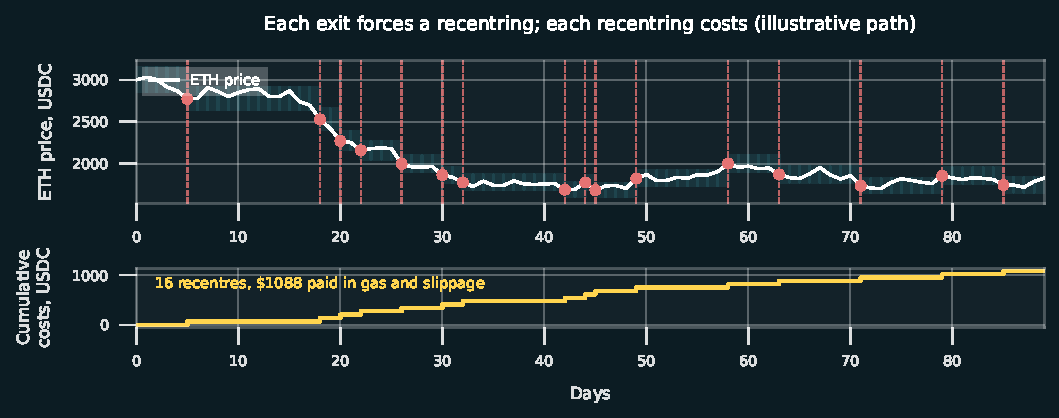
\includegraphics[width=0.92\linewidth]{figures/decision_path.pdf}
\caption{Why acting is a decision rather than a rule. An illustrative price
path with a $\pm5\%$ band: each exit forces a recentring, and each recentring
adds gas and slippage to a cost that only ever grows. The path is illustrative
and the costs are simplified; the study charges per-block gas and slippage on
the inventory actually swapped.}
\label{fig:decisions}
\end{figure}
